% 2021年北京高考数学第17题：长方体与截面
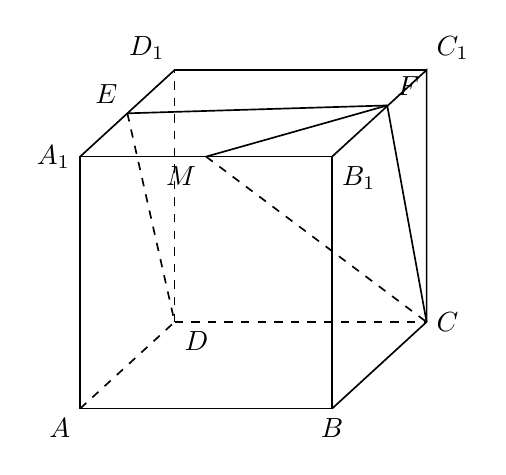
\begin{tikzpicture}[>=stealth,line width=0.6pt,font=\normalsize]
  \coordinate (A) at (0,0);
  \coordinate (B) at (3.2,0);
  \coordinate (C) at (4.4,1.1);
  \coordinate (D) at (1.2,1.1);
  \coordinate (A1) at (0,3.2);
  \coordinate (B1) at (3.2,3.2);
  \coordinate (C1) at (4.4,4.3);
  \coordinate (D1) at (1.2,4.3);

  \coordinate (E) at (0.6,3.75);
  \coordinate (F) at (3.9,3.85);
  \coordinate (M) at (1.6,3.2);

  % 可见外框
  \draw (A) -- (B) -- (B1) -- (A1) -- cycle;
  \draw (B) -- (C) -- (C1) -- (B1);
  \draw (A1) -- (D1) -- (C1);

  % 顶面与侧面线
  \draw (E) -- (F);
  \draw (F) -- (C);
  \draw (M) -- (F);

  % 虚线不可见边与截面线
  \draw[dashed] (A) -- (D);
  \draw[dashed] (D) -- (C);
  \draw[dashed] (D) -- (D1);
  \draw[dashed] (E) -- (D);
  \draw[dashed] (M) -- (C);

  % 顶点标注
  \node[below left] at (A) {$A$};
  \node[below] at (B) {$B$};
  \node[right] at (C) {$C$};
  \node[below right] at (D) {$D$};
  \node[left] at (A1) {$A_1$};
  \node[below right] at (B1) {$B_1$};
  \node[above right] at (C1) {$C_1$};
  \node[above left] at (D1) {$D_1$};
  \node[above left] at (E) {$E$};
  \node[above right] at (F) {$F$};
  \node[below left] at (M) {$M$};
\end{tikzpicture}
